\documentclass[]{article}
\usepackage{lmodern}
\usepackage{amssymb,amsmath}
\usepackage{ifxetex,ifluatex}
\usepackage{fixltx2e} % provides \textsubscript
\ifnum 0\ifxetex 1\fi\ifluatex 1\fi=0 % if pdftex
  \usepackage[T1]{fontenc}
  \usepackage[utf8]{inputenc}
\else % if luatex or xelatex
  \ifxetex
    \usepackage{mathspec}
  \else
    \usepackage{fontspec}
  \fi
  \defaultfontfeatures{Ligatures=TeX,Scale=MatchLowercase}
\fi
% use upquote if available, for straight quotes in verbatim environments
\IfFileExists{upquote.sty}{\usepackage{upquote}}{}
% use microtype if available
\IfFileExists{microtype.sty}{%
\usepackage{microtype}
\UseMicrotypeSet[protrusion]{basicmath} % disable protrusion for tt fonts
}{}
\usepackage[margin=1in]{geometry}
\usepackage{hyperref}
\hypersetup{unicode=true,
            pdftitle={metasim-draft},
            pdfauthor={Charles T. Gray},
            pdfborder={0 0 0},
            breaklinks=true}
\urlstyle{same}  % don't use monospace font for urls
\usepackage{color}
\usepackage{fancyvrb}
\newcommand{\VerbBar}{|}
\newcommand{\VERB}{\Verb[commandchars=\\\{\}]}
\DefineVerbatimEnvironment{Highlighting}{Verbatim}{commandchars=\\\{\}}
% Add ',fontsize=\small' for more characters per line
\usepackage{framed}
\definecolor{shadecolor}{RGB}{248,248,248}
\newenvironment{Shaded}{\begin{snugshade}}{\end{snugshade}}
\newcommand{\AlertTok}[1]{\textcolor[rgb]{0.94,0.16,0.16}{#1}}
\newcommand{\AnnotationTok}[1]{\textcolor[rgb]{0.56,0.35,0.01}{\textbf{\textit{#1}}}}
\newcommand{\AttributeTok}[1]{\textcolor[rgb]{0.77,0.63,0.00}{#1}}
\newcommand{\BaseNTok}[1]{\textcolor[rgb]{0.00,0.00,0.81}{#1}}
\newcommand{\BuiltInTok}[1]{#1}
\newcommand{\CharTok}[1]{\textcolor[rgb]{0.31,0.60,0.02}{#1}}
\newcommand{\CommentTok}[1]{\textcolor[rgb]{0.56,0.35,0.01}{\textit{#1}}}
\newcommand{\CommentVarTok}[1]{\textcolor[rgb]{0.56,0.35,0.01}{\textbf{\textit{#1}}}}
\newcommand{\ConstantTok}[1]{\textcolor[rgb]{0.00,0.00,0.00}{#1}}
\newcommand{\ControlFlowTok}[1]{\textcolor[rgb]{0.13,0.29,0.53}{\textbf{#1}}}
\newcommand{\DataTypeTok}[1]{\textcolor[rgb]{0.13,0.29,0.53}{#1}}
\newcommand{\DecValTok}[1]{\textcolor[rgb]{0.00,0.00,0.81}{#1}}
\newcommand{\DocumentationTok}[1]{\textcolor[rgb]{0.56,0.35,0.01}{\textbf{\textit{#1}}}}
\newcommand{\ErrorTok}[1]{\textcolor[rgb]{0.64,0.00,0.00}{\textbf{#1}}}
\newcommand{\ExtensionTok}[1]{#1}
\newcommand{\FloatTok}[1]{\textcolor[rgb]{0.00,0.00,0.81}{#1}}
\newcommand{\FunctionTok}[1]{\textcolor[rgb]{0.00,0.00,0.00}{#1}}
\newcommand{\ImportTok}[1]{#1}
\newcommand{\InformationTok}[1]{\textcolor[rgb]{0.56,0.35,0.01}{\textbf{\textit{#1}}}}
\newcommand{\KeywordTok}[1]{\textcolor[rgb]{0.13,0.29,0.53}{\textbf{#1}}}
\newcommand{\NormalTok}[1]{#1}
\newcommand{\OperatorTok}[1]{\textcolor[rgb]{0.81,0.36,0.00}{\textbf{#1}}}
\newcommand{\OtherTok}[1]{\textcolor[rgb]{0.56,0.35,0.01}{#1}}
\newcommand{\PreprocessorTok}[1]{\textcolor[rgb]{0.56,0.35,0.01}{\textit{#1}}}
\newcommand{\RegionMarkerTok}[1]{#1}
\newcommand{\SpecialCharTok}[1]{\textcolor[rgb]{0.00,0.00,0.00}{#1}}
\newcommand{\SpecialStringTok}[1]{\textcolor[rgb]{0.31,0.60,0.02}{#1}}
\newcommand{\StringTok}[1]{\textcolor[rgb]{0.31,0.60,0.02}{#1}}
\newcommand{\VariableTok}[1]{\textcolor[rgb]{0.00,0.00,0.00}{#1}}
\newcommand{\VerbatimStringTok}[1]{\textcolor[rgb]{0.31,0.60,0.02}{#1}}
\newcommand{\WarningTok}[1]{\textcolor[rgb]{0.56,0.35,0.01}{\textbf{\textit{#1}}}}
\usepackage{longtable,booktabs}
\usepackage{graphicx,grffile}
\makeatletter
\def\maxwidth{\ifdim\Gin@nat@width>\linewidth\linewidth\else\Gin@nat@width\fi}
\def\maxheight{\ifdim\Gin@nat@height>\textheight\textheight\else\Gin@nat@height\fi}
\makeatother
% Scale images if necessary, so that they will not overflow the page
% margins by default, and it is still possible to overwrite the defaults
% using explicit options in \includegraphics[width, height, ...]{}
\setkeys{Gin}{width=\maxwidth,height=\maxheight,keepaspectratio}
\IfFileExists{parskip.sty}{%
\usepackage{parskip}
}{% else
\setlength{\parindent}{0pt}
\setlength{\parskip}{6pt plus 2pt minus 1pt}
}
\setlength{\emergencystretch}{3em}  % prevent overfull lines
\providecommand{\tightlist}{%
  \setlength{\itemsep}{0pt}\setlength{\parskip}{0pt}}
\setcounter{secnumdepth}{0}
% Redefines (sub)paragraphs to behave more like sections
\ifx\paragraph\undefined\else
\let\oldparagraph\paragraph
\renewcommand{\paragraph}[1]{\oldparagraph{#1}\mbox{}}
\fi
\ifx\subparagraph\undefined\else
\let\oldsubparagraph\subparagraph
\renewcommand{\subparagraph}[1]{\oldsubparagraph{#1}\mbox{}}
\fi

%%% Use protect on footnotes to avoid problems with footnotes in titles
\let\rmarkdownfootnote\footnote%
\def\footnote{\protect\rmarkdownfootnote}

%%% Change title format to be more compact
\usepackage{titling}

% Create subtitle command for use in maketitle
\providecommand{\subtitle}[1]{
  \posttitle{
    \begin{center}\large#1\end{center}
    }
}

\setlength{\droptitle}{-2em}

  \title{metasim-draft}
    \pretitle{\vspace{\droptitle}\centering\huge}
  \posttitle{\par}
    \author{Charles T. Gray}
    \preauthor{\centering\large\emph}
  \postauthor{\par}
      \predate{\centering\large\emph}
  \postdate{\par}
    \date{04/05/2019}


\begin{document}
\maketitle

\hypertarget{vignette-text}{%
\section{vignette text}\label{vignette-text}}

\hypertarget{preamble}{%
\subsection{preamble}\label{preamble}}

\begin{Shaded}
\begin{Highlighting}[]
\CommentTok{# packages used in this paper}
\KeywordTok{library}\NormalTok{(metasim)}
\KeywordTok{library}\NormalTok{(tidyverse)}
\KeywordTok{library}\NormalTok{(patchwork)}


\CommentTok{# for reproducibility}
\KeywordTok{set.seed}\NormalTok{(}\DecValTok{38}\NormalTok{)}
\end{Highlighting}
\end{Shaded}

\hypertarget{introduction}{%
\subsection{introduction}\label{introduction}}

\texttt{metasim::} aims to lower the programmatic barrier to running
simulation experiments on meta-analysis estimators for the effect, or
variance of the effect, of interest. The intended audience of this
package are practicing scientists who wish to experiment to see how
their chosen estimator works under specific conditions, but who are not
necessarily computational mathematicians.

Frequently, scientists wish to verify their results, and, in particular,
that broad findings presented in literature hold for their particular
context. For example, perhaps an estimator works well for some sample
sizes and not others? For symmetric distributions, such as normal or
Cauchy, but not asymmetric distributions, such as exponential and
Pareto? Given practical and computational limitations, it is foregone
that not every case will have been considered in the literature. An
estimator is, after all, an algorithm, and susceptible to the no free
lunch principle (Wolpert and Macready 1997), wherein no algorithm is
optimised for all use cases.

The \texttt{metasim::} package was developed to test an estimator for
the variance of the sample median under meta-analysis. Given a
comparison was required, there is a high risk of repetitive code. And
this, too, creates a barrier for scientists whose primary discipline is
not programming. The more lines of repeated code, the more likely a
small mistake will cause the entire analysis algorithm to grind to a
halt. This is not insurmountable, but it \emph{is} time consuming.
Frequently the code was functional at the time of publication, but in
the meantime the author has made some small change in the code and it no
longer runs without debugging. This package aims to assist in smoothing
the inevitable debugging process that accompanies the simulation of
meta-analysis data.

todo: As open software, it is anticipated that \texttt{metasim::}

Consider - todo: use an example from Bland (Bland 2014) comparison paper
performs well for some sample sizes and not others.

\hypertarget{opinionated-bit}{%
\subsubsection{opinionated bit}\label{opinionated-bit}}

todo: not sure where this section goes

This package is an \emph{opinionated} algorithm (Parker 2017), in that
todo:

By integrating the output of the results todo:

Consider - three starting papers (Bland 2014; Hozo, Djulbegovic, and
Hozo 2005; Wan et al. 2014) + example dataset (Barros Pinheiro et al.
2012) of motivating problem, these were not written by statisticians.
Thus, it's okay for software to be opinionated. And indeed, we must, as
methodologists, make necessary choices about presentation and
implementation that carry the value judgement of opinion. There are
often multiple ways to solve a problem, and it is not always helpful to
provide all possible solutions. Often the end-user wishes to find a
useful guide.

todo: sweet spot between clippy-like interfaces and hard code (say,
traversing the CRAN guidebook thingies that I've never even looked at
for meta-analysis) - indeed, this is what the meta-verse aims to
do\ldots{}

\hypertarget{the-package-in-a-glance}{%
\subsection{the package in a glance}\label{the-package-in-a-glance}}

This package was

An advantage with standardised results, whatever they may be

\hypertarget{test-an-estimator}{%
\subsection{test an estimator}\label{test-an-estimator}}

This algorithm tests an estimator for the variance of the sample mean or
median through measuring \emph{coverage probability}, the proportion of
confidence intervals produced from the simulated data, or meta-analyses
of the simulated data.

In this case, we will assume an expected proportion
\(n_I / (n_C + n_I)\) of the intervention group, and how much 90 per
cent of proportions will deviate.

todo: rho is not what I think it is - need to redefine

Set expected p and its error. Let us assume there is equal division of
the total sample size for the \(k\)\emph{th} study.

\begin{Shaded}
\begin{Highlighting}[]
\NormalTok{p <-}\StringTok{ }\FloatTok{0.5} 
\NormalTok{p_error <-}\StringTok{ }\FloatTok{0.1}   
\end{Highlighting}
\end{Shaded}

\begin{Shaded}
\begin{Highlighting}[]
\KeywordTok{rho_plot}\NormalTok{(p, p_error)}
\end{Highlighting}
\end{Shaded}

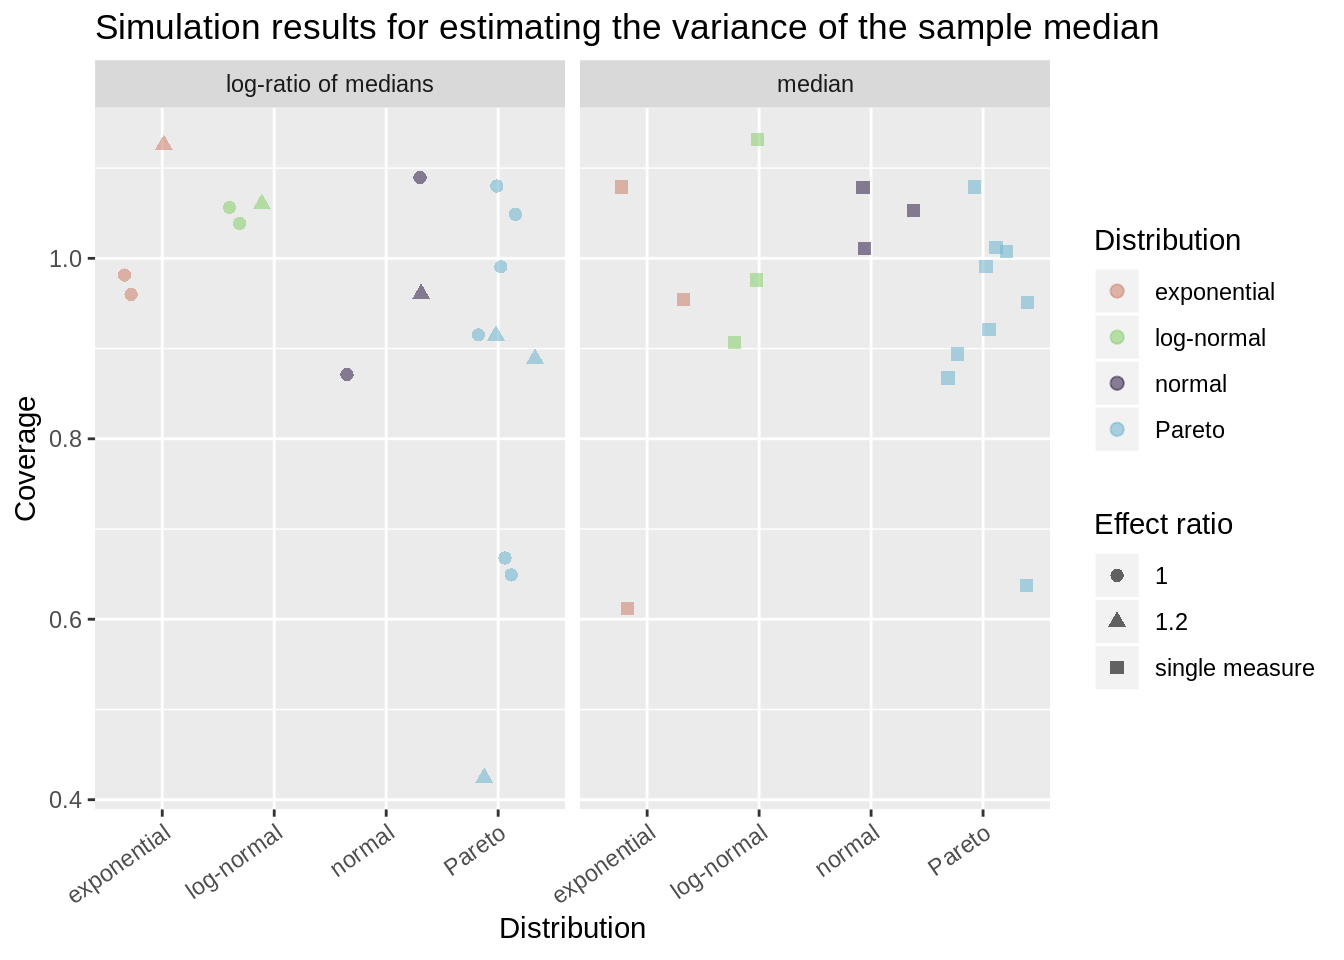
\includegraphics{metasim-draft_files/figure-latex/unnamed-chunk-2-1.pdf}

\hypertarget{sample-sizes}{%
\subsection{sample sizes}\label{sample-sizes}}

Different experimental designs require different divisions of sample
size, and there is a

\hypertarget{create-parameter-estimators}{%
\subsection{create parameter
estimators}\label{create-parameter-estimators}}

Here we define \(\rho\), the expected value of the proportion for the
intervention group. An expected value of \(\rho = 0.5\) would indicate
equal division between control and intervention group.

It stands to reason that there would be expected variance, in the
proportion \(\rho\) of the study's total sample size \(N\) allocated to
the intervention group \(n_i\). We define \texttt{epsilon}
\(:= \varepsilon\), the proportional deviation we allow for 90 per cent
of the combined intervention and control sample size, \(n_I + n_C = N\).

We assume the proportion \(p\) of the total sample size \(N\) allocated
to the intervention group follows a beta distribution,
\(p \sim \mathrm{Beta}(\alpha, \beta)\).

With these values, we can combine the expected value \(\rho\) of \(p\)
with its error \(\varepsilon\) to solve for the parameters of the beta
distribution.

Via Chebyshev's inequality, we have

\[
1 - \frac{\sigma^2}{\varepsilon^2} = 0.9
\]

where \(\sigma^2\) denotes \(\mathrm{Var}(p)\).

Then, as \(\mu\) is also known, we can find the parameters in terms of
the expected value \(\rho\) of \(p\) and its variation \(\varepsilon\),
given.

\[
\alpha := \rho \cdot (10\rho^2/\varepsilon^2 \cdot (1/\rho - 1) - 1)
\] \[
\beta := \frac \alpha \rho (1 - \rho).
\]

The \texttt{rho\_plot} function of \texttt{metasim::} provides a tool
for visually understanding the data will be sampled for the proportion
\(\rho\) of \(N\) allocated to the intervention group, based on the
assumptions, \(\mu\) and \(\varepsilon\).

\begin{Shaded}
\begin{Highlighting}[]
\CommentTok{# collect plots for different expected values}
\NormalTok{plots <-}\StringTok{ }\KeywordTok{map2}\NormalTok{(}\KeywordTok{list}\NormalTok{(}\FloatTok{0.5}\NormalTok{, }\FloatTok{0.2}\NormalTok{, }\FloatTok{0.8}\NormalTok{, }\FloatTok{0.3}\NormalTok{), }\KeywordTok{list}\NormalTok{(}\FloatTok{0.2}\NormalTok{, }\FloatTok{0.01}\NormalTok{, }\FloatTok{0.1}\NormalTok{, }\FloatTok{0.25}\NormalTok{), rho_plot)}

\CommentTok{# patchwork example plots}
\NormalTok{plots[[}\DecValTok{1}\NormalTok{]] }\OperatorTok{+}\StringTok{ }\NormalTok{plots[[}\DecValTok{2}\NormalTok{]] }\OperatorTok{+}\StringTok{ }\NormalTok{plots[[}\DecValTok{3}\NormalTok{]] }\OperatorTok{+}\StringTok{ }\NormalTok{plots[[}\DecValTok{4}\NormalTok{]]}
\end{Highlighting}
\end{Shaded}

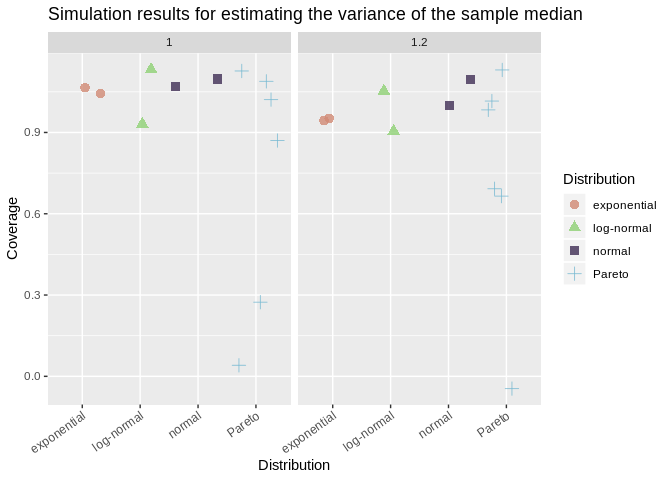
\includegraphics{metasim-draft_files/figure-latex/unnamed-chunk-3-1.pdf}

\hypertarget{sampling-the-data}{%
\subsection{sampling the data}\label{sampling-the-data}}

\hypertarget{assumptions}{%
\subsubsection{assumptions}\label{assumptions}}

Let

\begin{itemize}
\tightlist
\item
  \(j \in \{I, C\}\) for intervention and control groups,
\item
  \(k \in K\) studies,
\item
  \(i \in 1, \dots, n_{jk}\) sample size for the \(j\)\emph{th} group
  and \(k\)\emph{th} study
\item
  \(m_{jk}\) the sample median for the \(j\)\emph{th} group and
  \(k\)\emph{th} study
\item
  \(v_j\) the population median for the \(j\)\emph{th} group
\item
  \(x_{jki}\) denote the \(i\)\emph{th} observation for the
  \(j\)\emph{th} group and \(k\)\emph{th} study
\end{itemize}

Assume

\begin{itemize}
\tightlist
\item
  \(x_{jki} \sim h(\bar \varphi_{jk})\), where \(h\) is a probability
  distribution and \(\bar \varphi_{jk}\) denotes the set of parameters
  associated with \(h\) for the \(j\)\emph{th} group and \(k\)\emph{th}
  study
\item
  \(v_j\) is the median of the distribution \(h(\bar \varphi_j)\)
\end{itemize}

We assume the log-ratio of sample medians can be thought of in terms of
the log-ratio of true medians, \[
\log (m_{Ik}/m_{Ck}) = \log(\nu_I/\nu_C) + \gamma_k
\] with some deviation associated with the variation
\(\gamma_k \sim N(0, \tau^2)\) for the \(k\)\emph{th} study and sampling
error \(\varepsilon_k \sim N(0, \psi^2)\).

For simplicity, we assume all but the first parameter of \(h\) are equal
across for all \(K\) studies, and allow the first parameter to vary
according for the \(j\)\emph{th} group of the \(k\)\emph{th} study.

\hypertarget{first-parameter-derivations}{%
\subsubsection{first parameter
derivations}\label{first-parameter-derivations}}

\hypertarget{normal}{%
\paragraph{normal}\label{normal}}

Suppose \(x_{jki} \sim N(\mu_{jk}, \sigma_{jk})\) where the median
\(\nu_j\) denotes the median of \(N(\mu_j, \sigma_j)\).

For simplicity, we assume \(\sigma_j = \sigma = \sigma_{jk}\).

We wish to find \(\mu_{jk}\) in terms of \(\mu_j\) and \(\sigma^2\),
\(\gamma_k\), and \(\varepsilon_k\).

Since \(x_{jki} \sim N(\mu_{jk}, \sigma)\), we have
\(\nu_{jk} = \mu_{jk}\) and \(\nu_j = \mu_j\), then

\begin{align*}
\log(m_{Ik}/m_{Ck}) &= \log(\nu_I/\nu_C) + \gamma_k \\
\implies \log(\mu_{Ik}/\mu_{Ck}) &= \log(\mu_I/\mu_C) + \gamma_k\\
\implies \log\mu_{Ik} - \log\mu_{Ck} &= \log\mu_I - \log\mu_C + 2\gamma_k/2 + 2\varepsilon_k/2\\
\implies \log\mu_{jk} &= \log\mu_j + \gamma_k/2 + \varepsilon_k/2\\
\implies \mu_{jk} &= \mu_j e^{\frac{\gamma_k}{2}}.
\end{align*}

\hypertarget{log-normal}{%
\paragraph{log-normal}\label{log-normal}}

Suppose \(x_{jki} \sim \log N(\mu_{jk}, \sigma_{jk})\), where \(\nu_j\)
denotes the median of \(\log N(\mu_j, \sigma_j)\).

Then, \(\nu_{jk} = \exp(\mu{jk})\) and \(\nu_j = \exp(\mu_j)\).

For simplicity, we assume \(\sigma_j = \sigma = \sigma_{jk}\). So,

\begin{align*}
\log(m_{Ik}/m_{Ck}) &= \log(\nu_I/\nu_C) + \gamma_k \\
\implies \log(\exp(\mu_{Ik})) - \log(\exp(\mu_{Ck})) &= \log(\exp(\mu_I)) - \log(\exp(\mu_C)) + 2\gamma_k/2 + 2\varepsilon_k/2\\
\implies \mu_{jk} &= \mu_j + \gamma_k/2 + \varepsilon_k/2.
\end{align*}

\noindent \textbf{Another way to look at it:} the aim is to add a random
effect to the log ratio of medians. Using notations above, we want
\(\log(\nu_{1k}/\nu_{2k}) + \gamma_k\) which is equal to
\(\log(\nu_{1k}) - log(\nu_{2k}) + \gamma_k = \mu_{1k} - \mu_{2k} + \gamma_k\).
So the question is, when we are going to sample from the log-normal
distributions for each group then what do we do with the random effect?
One way is to split it between the two which gives
\[(\mu_{1k} + \gamma_k/2) - (\mu_{2k} - \gamma_k/2).\] Therefore we
simulate the \(x_{1ki}\)s from the LN\((\mu_{1k} + \gamma_k/2, \sigma)\)
distribution and the \(x_{2ki}\)s from the
LN\((\mu_{2k} - \gamma_k/2, \sigma)\) distribution. This is similar to
what is above, but where (i) note the \(-\gamma_k/2\) for the second
group, and (ii) no sampling error, \(\epsilon_k\). The sampling error is
to account for the sample median being as estimator of the median. So it
shouldn't be used in the sampling process.

\hypertarget{pareto}{%
\paragraph{pareto}\label{pareto}}

Suppose \(x_{jki} \sim \mathrm{Pareto}(\theta_{jk}, \alpha_{jk})\) where
\(\nu_j\) denotes the median of
\(\mathrm{Pareto}(\theta_{j}, \alpha_{j})\).

Then \(\nu_{jk} = \theta_{jk} \sqrt[\alpha_{jk}]2\) and
\(\nu_{j} = \theta_{j} \sqrt[\alpha_{j}]2\).

For simplicity, we assume \(\alpha_{jk} = \alpha = \alpha_j\). Then,
\begin{align*}
\log(m_{Ik}/m_{Ck}) &= \log(\nu_I/\nu_C) + \gamma_k \\
\implies \log(\theta_{Ik} \sqrt[\alpha_{Ik}]2/\theta_{Ck} \sqrt[\alpha_{Ck}]2) &= \log(\theta_{I} \sqrt[\alpha_{I}]2/\theta_{C} \sqrt[\alpha_{C}]2) + 2\gamma_k/2 + 2\varepsilon_k/2\\
\implies \log(\theta_{jk}\sqrt[\alpha_{jk}]2)  &= \log(\theta_{j} \sqrt[\alpha_{j}]2) + \gamma_k/2 + \varepsilon_k/2\\
\implies \theta_{jk}\sqrt[\alpha_{jk}]2 &= \theta_{j} \sqrt[\alpha_{j}]2 e^{\frac{\gamma_k}{2}}. 
\end{align*}

And, since \(\alpha_{jk} = \alpha = \alpha_j\), we have \[
\theta_{jk} = \theta_j e^{\frac{\gamma_k}{2}}.
\]

\hypertarget{exponential}{%
\paragraph{exponential}\label{exponential}}

Suppose \(x_{jki} \sim \exp(\lambda_{jk})\) where \(\nu_j\) denotes the
median of \(\exp(\lambda_j)\).

Then \(m_{jk} = \log2/\lambda_{jk}\) and \(\nu_j = \log2/\lambda_j\).
So,

\begin{align*}
\log(m_{Ik}/m_{Ck}) &= \log(\nu_I/\nu_C) + \gamma_k \\
\implies \log\lambda_{Ck} - \log\lambda_{Ik} &= \log\lambda_C - \log\lambda_I + 2\gamma_k/2 + 2\varepsilon_k/2\\
\implies \log\lambda_{jk} &= \log\lambda_j + \gamma_k/2 + \varepsilon_k/2\\
\implies \lambda_{jk} &= \lambda_j e^{\frac{\gamma_k}{2}}.
\end{align*}

\hypertarget{simulation-parameters}{%
\subsubsection{simulation parameters}\label{simulation-parameters}}

Since we're interested in simulating for differences between the group
medians, and no differnce between the group medians, we set a
proportional difference \(p\) between the medians, which defaults to 1
(no difference).

We set the control parameters \(\bar \varphi_C\) as simulation-level
parameter, from which we derive a control median \(\nu_C\) and calculate
the intervention median, \[
\frac{\nu_I}{\nu_C} = p \implies \nu_I = p\nu_C.
\]

\hypertarget{normal-1}{%
\paragraph{normal}\label{normal-1}}

Since \(\nu_j = \mu_j\), for \(N(\mu_j, \sigma^2)\),

\[
\nu_I = p \nu_C \implies \mu_I = p \mu_C.
\]

\hypertarget{log-normal-1}{%
\paragraph{log-normal}\label{log-normal-1}}

Since \(\nu_j = \exp(\mu_j)\), for \(\log N(\mu_j, \sigma_j)\),

\[
\nu_I = p \nu_C \implies \exp(\mu_I) = p \exp(\mu_C) \implies \mu_I = \log p + \mu_C. 
\]

\hypertarget{pareto-1}{%
\paragraph{pareto}\label{pareto-1}}

Since \(\nu_j = \theta_j \sqrt[\alpha_j]2\), for
\(\mathrm{Pareto}(\theta_j, \alpha_j)\),

\[
\nu_I = p \nu_C \implies \theta_I \sqrt[\alpha_I]2 = p \theta_C \sqrt[\alpha_C]2 \implies \theta_I = p\theta_C.
\]

\hypertarget{exponential-1}{%
\paragraph{exponential}\label{exponential-1}}

Since \(\nu_j = \log2/\lambda_j\), for \(\exp(\lambda_j)\),

\[
\nu_I = p \nu_C \implies \log2/\lambda_I = \log2/\lambda_C \implies \lambda_I = \lambda_C/p. 
\]

\hypertarget{applications}{%
\subsection{applications}\label{applications}}

\hypertarget{meta-analysis-of-medians-metamed}{%
\subsubsection{meta-analysis of medians
\{metamed\}}\label{meta-analysis-of-medians-metamed}}

The \texttt{metasim::} package began as a script to solve this
particular problem, and so it is currently the default simulation
parameter set for \texttt{metasims()}.

\hypertarget{the-problem}{%
\paragraph{the problem}\label{the-problem}}

\hypertarget{simulation-parameters-1}{%
\paragraph{simulation parameters}\label{simulation-parameters-1}}

In order to compare the performance of the estimator, we wished to
consider a number of different constraints.

\begin{verbatim}
##  [1] "single_study"   "measure"        "measure_spread" "distributions" 
##  [5] "k"              "tau2_true"      "effect_ratio"   "min_n"         
##  [9] "max_n"          "prop"           "prop_error"     "trials"        
## [13] "trial_fn"       "beep"           "progress"       ""
\end{verbatim}

\begin{itemize}
\tightlist
\item
  \(k =\) 3, 7, 10 studies
\item
  \(\tau^2 =\) 0, 0.2, 0.4 variation between studies
\item
  constrain the smallest and largest size sample, from 20 , to 200.
\item
  compare how the estimator performs for whether there is no difference,
  between the control and intervention group, of the two measures of
  interest, and when there is; with the ratio of effects
  \(\rho = \nu_I / \nu_C =\) 1, 1.2
\item
  sample from symmetric (normal distribution) and asymmetric
  (log-normal, exponential) underlying distributions, from any number of
  a parameter sets.
\item
  the expected proportion the intervention group, defaulting to 0.5 and
  what difference from the 0.1 difference 90\% of other proportions fall
  within.
\end{itemize}

There is scope to extend the number of distributions in future releases
of \texttt{metasim::}. Furthermore, the question of the optimal
selection of simulation parameter sets remains for future work. For
example, incorporating elements from experimental design (Steponavic et
al. 2016) into the construction of the simulation parameter set.

A set of default parameters is exported as a data object
\texttt{default\_parameters} in \texttt{metasim::}.

\begin{longtable}[]{@{}ll@{}}
\toprule
distribution & parameters\tabularnewline
\midrule
\endhead
normal & 2, 0.3\tabularnewline
exponential & 2\tabularnewline
Pareto & 3, 3\tabularnewline
Pareto & 2, 1\tabularnewline
Pareto & 0.5, 1\tabularnewline
log-normal & 1, 0.3\tabularnewline
\bottomrule
\end{longtable}

\hypertarget{default-distributions}{%
\paragraph{default distributions}\label{default-distributions}}

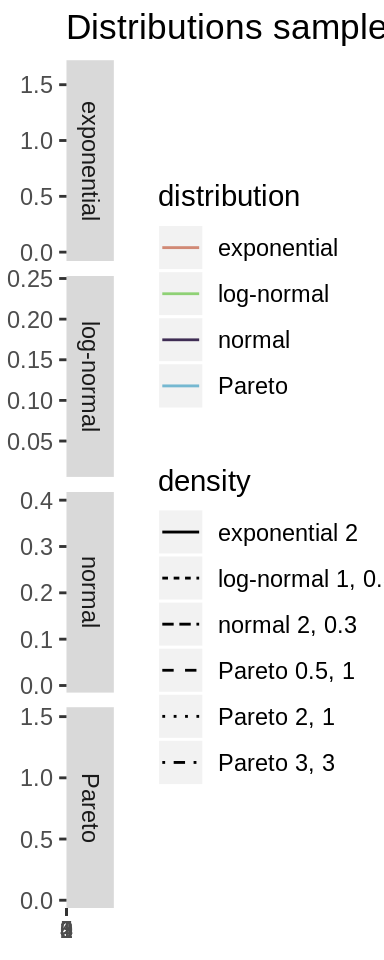
\includegraphics{metasim-draft_files/figure-latex/distribution plots-1.pdf}

\hypertarget{ratio-plots}{%
\paragraph{ratio plots}\label{ratio-plots}}

\hypertarget{single-study-simulation}{%
\paragraph{single-study simulation}\label{single-study-simulation}}

\begin{Shaded}
\begin{Highlighting}[]
\NormalTok{single_sim <-}\StringTok{ }\KeywordTok{metasims}\NormalTok{(}
  \DataTypeTok{trials =}\NormalTok{ params}\OperatorTok{$}\NormalTok{trials,}
  \DataTypeTok{progress =} \OtherTok{FALSE}\NormalTok{, }
  \DataTypeTok{single_study =} \OtherTok{TRUE}\NormalTok{)}

\CommentTok{# generate a caption}
\NormalTok{single_sim }\OperatorTok
\StringTok{  }\KeywordTok{mutate}\NormalTok{(}\DataTypeTok{distribution =} \KeywordTok{map_chr}\NormalTok{(rdist, dist_name)) }\OperatorTok
\StringTok{  }\KeywordTok{ggplot}\NormalTok{(}\KeywordTok{aes}\NormalTok{(}\DataTypeTok{x =}\NormalTok{ distribution, }\DataTypeTok{y =}\NormalTok{ coverage)) }\OperatorTok{+}
\StringTok{  }\KeywordTok{geom_point}\NormalTok{(}
         \DataTypeTok{position =} \StringTok{"jitter"}\NormalTok{,}
         \KeywordTok{aes}\NormalTok{(}\DataTypeTok{colour =}\NormalTok{ distribution, }\DataTypeTok{shape =} \KeywordTok{as.character}\NormalTok{(effect_ratio)),}
         \DataTypeTok{alpha =} \FloatTok{0.8}\NormalTok{,}
         \DataTypeTok{size =} \DecValTok{3}
\NormalTok{       ) }\OperatorTok{+}
\StringTok{  }\KeywordTok{scale_shape_discrete}\NormalTok{(}\DataTypeTok{name =} \StringTok{"Effect ratio"}\NormalTok{) }\OperatorTok{+}
\StringTok{  }\NormalTok{hrbrthemes}\OperatorTok{::}\KeywordTok{scale_colour_ipsum}\NormalTok{(}\DataTypeTok{name =} \StringTok{"Distribution"}\NormalTok{) }\OperatorTok{+}
\StringTok{  }\KeywordTok{labs}\NormalTok{(}
    \DataTypeTok{x =} \StringTok{"Distribution"}\NormalTok{,}
       \DataTypeTok{y =} \StringTok{"Coverage"}\NormalTok{,}
    \DataTypeTok{title =} \KeywordTok{str_wrap}\NormalTok{(}
      \StringTok{"Simulation results for estimating the variance of the sample median"}
\NormalTok{    ),}
    \DataTypeTok{caption =}\NormalTok{ single_sim_caption }\OperatorTok\StringTok{ }\KeywordTok{str_wrap}\NormalTok{(}\DataTypeTok{width =}\NormalTok{ cap_width)}
\NormalTok{  ) }\OperatorTok{+}\StringTok{ }\KeywordTok{theme}\NormalTok{(}
    \DataTypeTok{axis.text.x =} \KeywordTok{element_text}\NormalTok{(}
      \DataTypeTok{angle =} \DecValTok{35}\NormalTok{,}
      \DataTypeTok{hjust =} \DecValTok{1}\NormalTok{,}
      \DataTypeTok{vjust =} \DecValTok{1}
\NormalTok{    ),}
    \DataTypeTok{plot.caption =} \KeywordTok{element_text}\NormalTok{(}\DataTypeTok{hjust =} \DecValTok{0}\NormalTok{, }\DataTypeTok{margin =} \KeywordTok{margin}\NormalTok{(}\DataTypeTok{t =} \DecValTok{10}\NormalTok{))}
\NormalTok{  ) }
\end{Highlighting}
\end{Shaded}

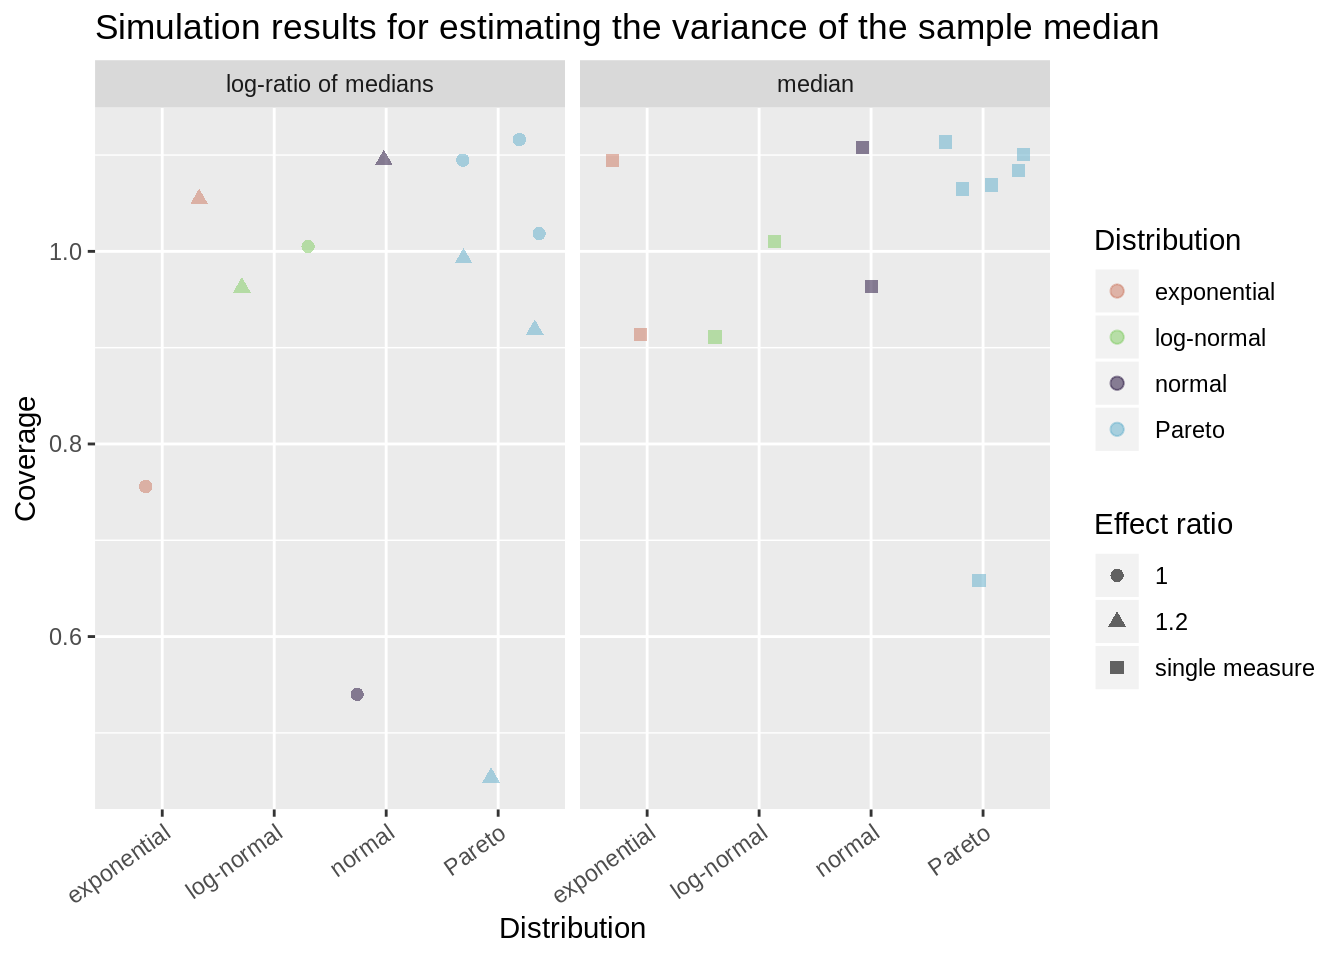
\includegraphics{metasim-draft_files/figure-latex/ss plot-1.pdf}

\begin{Shaded}
\begin{Highlighting}[]
\CommentTok{# ("visualisations/single-sim.svg")}
\end{Highlighting}
\end{Shaded}

\hypertarget{meta-analysis-simulation}{%
\paragraph{meta-analysis simulation}\label{meta-analysis-simulation}}

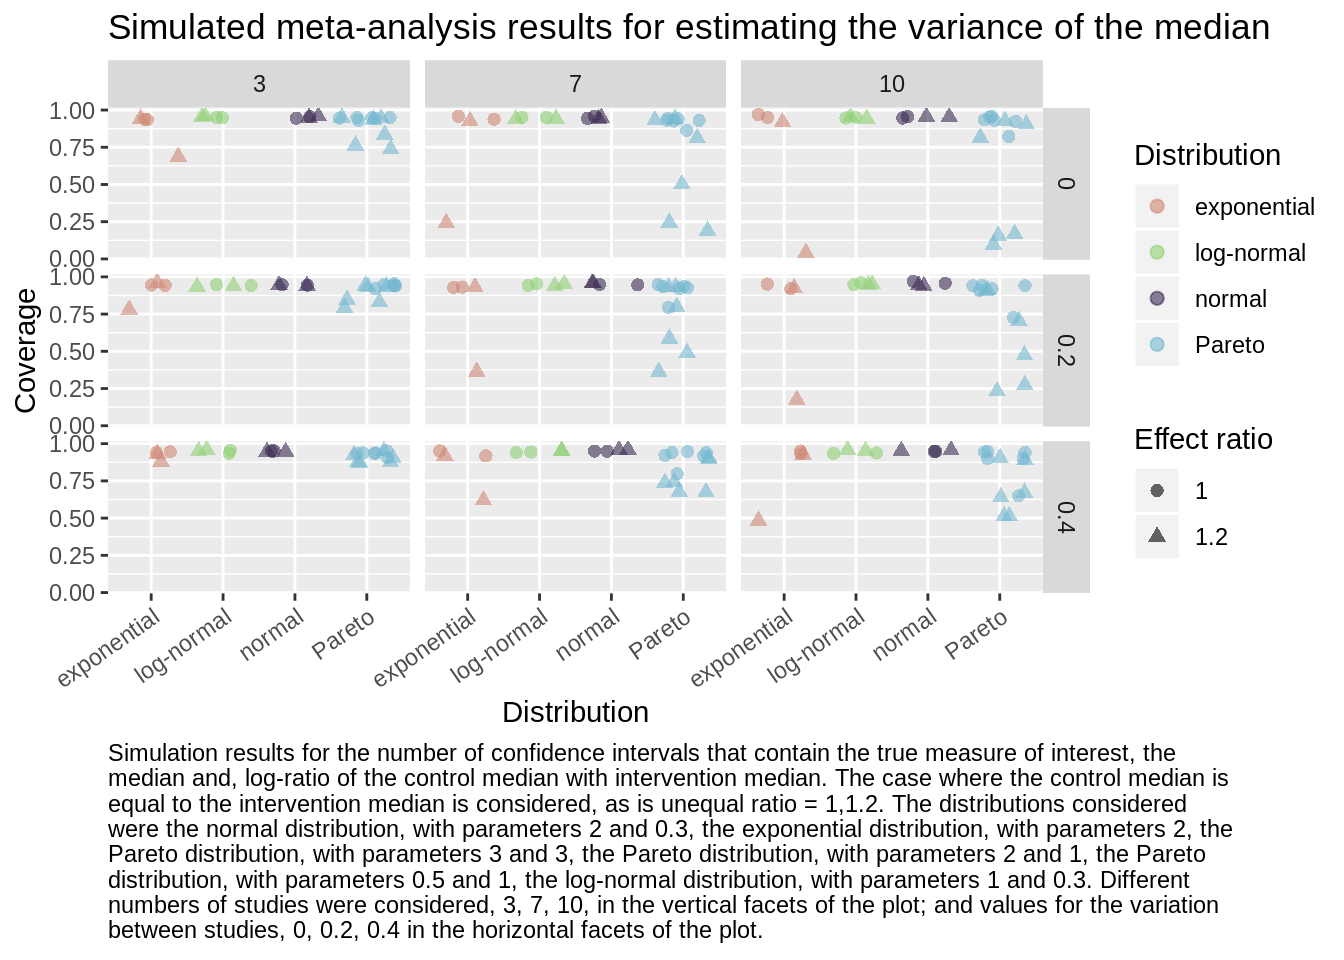
\includegraphics{metasim-draft_files/figure-latex/ma plot-1.pdf}

\hypertarget{references}{%
\subsection*{references}\label{references}}
\addcontentsline{toc}{subsection}{references}

\hypertarget{refs}{}
\leavevmode\hypertarget{ref-pinheiro_d-dimer_2012}{}%
Barros Pinheiro, Melina de, Daniela Rezende Garcia Junqueira, Fernanda
Fonseca Coelho, Let\a'ıcia G. Freitas, Maria G. Carvalho, Karina Braga
Gomes, and Luci Maria Santana Dusse. 2012. ``D-Dimer in Preeclampsia:
Systematic Review and Meta-Analysis.'' \emph{Clinica Chimica Acta;
International Journal of Clinical Chemistry} 414 (December): 166--70.
\url{https://doi.org/10.1016/j.cca.2012.08.003}.

\leavevmode\hypertarget{ref-bland_estimating_2014}{}%
Bland, Martin. 2014. ``Estimating Mean and Standard Deviation from the
Sample Size, Three Quartiles, Minimum, and Maximum.''
\emph{International Journal of Statistics in Medical Research} 4 (1):
57--64--64.
\url{http://lifescienceglobal.com/pms/index.php/ijsmr/article/view/2688}.

\leavevmode\hypertarget{ref-hozo_estimating_2005}{}%
Hozo, Stela Pudar, Benjamin Djulbegovic, and Iztok Hozo. 2005.
``Estimating the Mean and Variance from the Median, Range, and the Size
of a Sample.'' \emph{BMC Medical Research Methodology} 5 (1): 13.
\url{https://doi.org/10.1186/1471-2288-5-13}.

\leavevmode\hypertarget{ref-parker_opinionated_2017}{}%
Parker, Hilary. 2017. ``Opinionated Analysis Development.''
\emph{Preprint}. \url{https://doi.org/10.7287/peerj.preprints.3210v1}.

\leavevmode\hypertarget{ref-pardalos_sampling_2016}{}%
Steponavic, Ingrida, Mojdeh Shirazi-Manesh, Rob J. Hyndman, Kate
Smith-Miles, and Laura Villanova. 2016. ``On Sampling Methods for Costly
Multi-Objective Black-Box Optimization.'' In \emph{Advances in
Stochastic and Deterministic Global Optimization}, edited by Panos M.
Pardalos, Anatoly Zhigljavsky, and Julius Zilinskas, 107:273--96. Cham:
Springer International Publishing.
\url{https://doi.org/10.1007/978-3-319-29975-4_15}.

\leavevmode\hypertarget{ref-wan_estimating_2014}{}%
Wan, Xiang, Wenqian Wang, Jiming Liu, and Tiejun Tong. 2014.
``Estimating the Sample Mean and Standard Deviation from the Sample
Size, Median, Range and/or Interquartile Range.'' \emph{BMC Medical
Research Methodology} 14 (1): 135.
\url{https://doi.org/10.1186/1471-2288-14-135}.

\leavevmode\hypertarget{ref-wolpert_no_1997}{}%
Wolpert, D.H., and W.G. Macready. 1997. ``No Free Lunch Theorems for
Optimization.'' \emph{IEEE Transactions on Evolutionary Computation} 1
(1): 67--82. \url{https://doi.org/10.1109/4235.585893}.


\end{document}
